\question{}

\begin{ابجد}
\item برای بیشینه کردن تعداد برگ‌های قابل هرس، می‌توانیم به این طریق عمل کنیم: در زیردرخت سمت چپ، باید ابتدا یک مقدار برای $min_1$ مشخص شده باشد. پس باید دو برگ $x_1$ و $x_2$ را دیده باشیم تا مقدار $max_1$ مشخص شده باشد. اما می‌توان کاری کرد که با دیدن برگ $x_3$ مطمئن شویم که $max_2 \geq min_1$ و بتوانیم $x_4$ را هرس کنیم. پس باید:

\begin{equation*}
    x_3 \geq max(x_1, x_2)
\end{equation*}

در زیردرخت سمت راست، باید مقدار $max_3$ مشخص شده باشد تا $min_2$ مقدار اولیه گرفته باشد. برای اینکه بتوانیم باقی این زیردرخت (برگ‌های $x_7$ و $x_8$) را هرس کنیم، باید مقدار $max_3$ کمتر مساوی مقدار فعلی $max_0$ (که همان مقدار $min_1$ است) باشد. چون در این صورت مطمئن هستیم که $min_2$ مقدار بیشتر از $max_0$ نمی‌گیرد و بازیکن $max_0$ شاخه سمت راست را انتخاب نمی‌کند. بنابراین:

\begin{equation*}
    min_2 \leq max(x_5, x_6) \leq min_1 = max(x_1, x_2)
\end{equation*}

با توجه به موارد بالا، می‌توانیم درخت را به این شکل مقداردهی کنیم:

\begin{figure}[H]
    \centering
    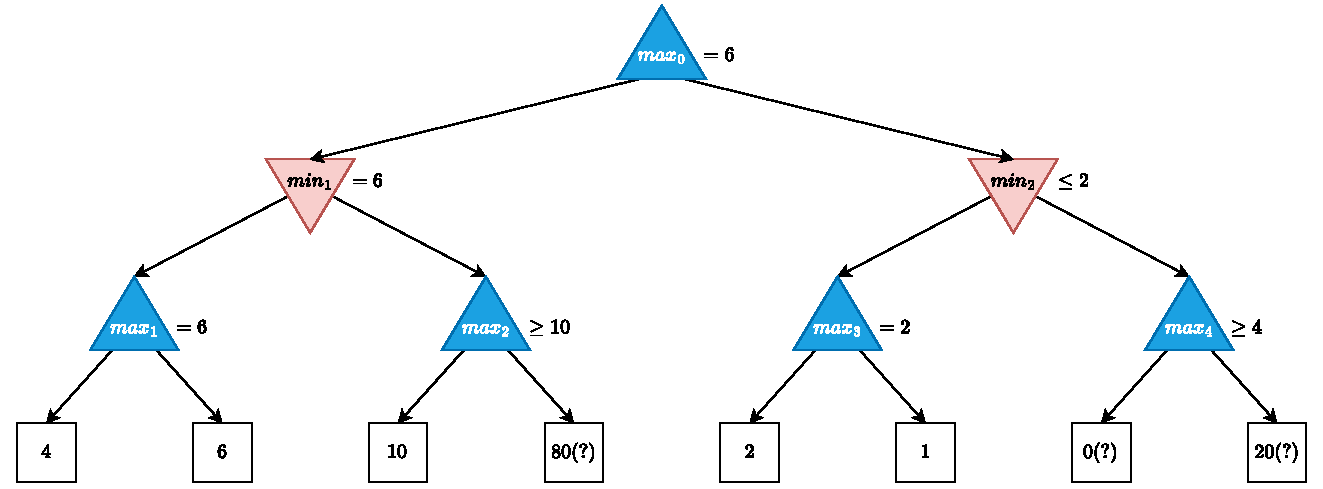
\includegraphics[width=0.8\textwidth]{assets/q4-A.pdf}
\end{figure}

\item می‌توان گفت برای این بخش، باید برعکس قسمت قبل عمل کنیم. با استدلال مشابه، در زیردرخت سمت چپ، باید $x_3 < max(x_1, x_2)$ تا نتوان $x_4$ را هرس کرد. همچنین باید $max(x_5, x_6) > min_1$ تا مجبور شویم زیردرخت $min_2$ را ببینیم. و در نهایت، باید $x_7 < max(x_5,x_6)$ تا نتوانیم $x_8$ را هرس کنیم. \\
با توجه به این موارد، می‌توان درخت را به این صورت مقداردهی کرد:

\begin{figure}[H]
    \centering
    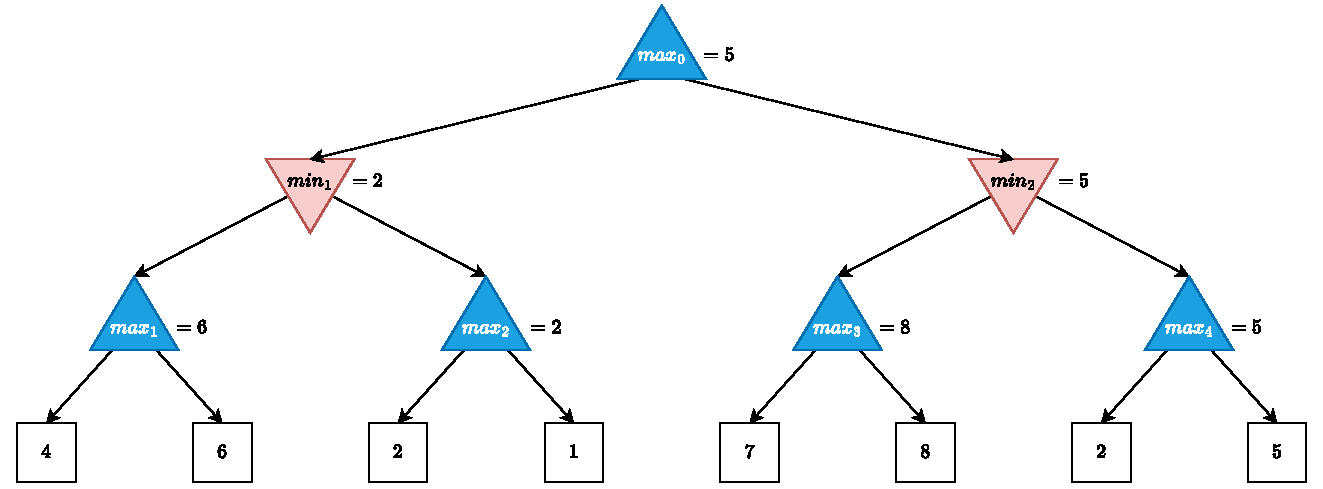
\includegraphics[width=0.8\textwidth]{assets/q4-B.pdf}
\end{figure}

\end{ابجد}